\documentclass[a4paper]{article}

% Set for specific document
\def\DOCTITLE{CSC3621 Coursework 1 Exercise 1}
\def\DOCAUTHOR{Dan Nixon (120263697)}
\def\DOCDATE{16/10/2015}

% Set document attributes
\title{\DOCTITLE}
\author{\DOCAUTHOR}
\date{\DOCDATE}

\usepackage{fullpage}
\usepackage{scrextend}
\usepackage{titlesec}
\usepackage{fancyhdr}
\usepackage{hyperref}
\usepackage[style=numeric-comp,natbib=true]{biblatex}
\usepackage[section]{placeins}
\usepackage{minted}
\usepackage{booktabs}

\addbibresource{CSC3621_CW1_Ex1_DanNixon.bib}

% Handle graphics correctly
\ifx\pdftexversion\undefined
\usepackage{graphicx}
% \usepackage[dvips]{graphicx}
\else
\usepackage[pdftex]{graphicx}
\DeclareGraphicsRule{*}{mps}{*}{}
\fi

% Setup headers and footers
\pagestyle{fancy}
\lhead{}
\chead{\DOCTITLE}
\rhead{}
\rfoot{\DOCDATE}
\cfoot{\thepage}
\lfoot{\DOCAUTHOR}

% Set header and footer sizes
\renewcommand{\headrulewidth}{0.4pt}
\renewcommand{\footrulewidth}{0.4pt}
\setlength{\headheight}{15.2pt}
\setlength{\headsep}{15.2pt}

\setlength{\textfloatsep}{0.1cm}

\begin{document}

\section{Frequency analysis of English plain text}

The frequency counter program is implemented in \texttt{FrequencyCounter.java}
(also using some dependencies from \texttt{Utils.java}) and can be executed
using the script \texttt{ex1\_run\_frequency\_analysis}.

The results of this analysis program are included in table
\ref{table:plain_text_frequency_analysis}, this shows published results from
analysis of Project Gutenberg Standard Selections \cite{gutenberg} as well as
results calculated by the program for the \texttt{pg1661.txt} file and RAL
Technical Report 2015 007 \cite{ral_tr_2015_007}.

\begin{table}[h]
  \centering
  \scriptsize
  \begin{tabular}{crrr}
    \toprule
    Character & Project Gutenberg & pg1661.txt & RAL-TR-2015-007 \\
    \midrule
    a         & 8.176\%           & 8.082\%    & 7.802\%         \\
    b         & 1.492\%           & 1.484\%    & 1.184\%         \\
    c         & 2.782\%           & 2.483\%    & 3.894\%         \\
    d         & 4.253\%           & 4.271\%    & 3.770\%         \\
    e         & 12.702\%          & 12.287\%   & 11.101\%        \\
    f         & 2.228\%           & 2.093\%    & 2.693\%         \\
    g         & 2.015\%           & 1.855\%    & 1.868\%         \\
    h         & 6.094\%           & 6.615\%    & 3.919\%         \\
    i         & 6.966\%           & 6.988\%    & 8.731\%         \\
    j         & 0.153\%           & 0.121\%    & 0.113\%         \\
    k         & 0.772\%           & 0.823\%    & 0.535\%         \\
    l         & 4.025\%           & 3.944\%    & 3.816\%         \\
    m         & 2.406\%           & 2.718\%    & 2.533\%         \\
    n         & 6.749\%           & 6.649\%    & 7.327\%         \\
    o         & 7.507\%           & 7.798\%    & 7.065\%         \\
    p         & 1.929\%           & 1.629\%    & 2.631\%         \\
    q         & 0.095\%           & 0.097\%    & 0.367\%         \\
    r         & 5.987\%           & 5.743\%    & 6.801\%         \\
    s         & 6.327\%           & 6.254\%    & 6.664\%         \\
    t         & 9.056\%           & 9.059\%    & 10.557\%        \\
    u         & 2.758\%           & 3.049\%    & 2.766\%         \\
    v         & 0.978\%           & 1.022\%    & 0.918\%         \\
    w         & 2.361\%           & 2.574\%    & 1.253\%         \\
    x         & 0.150\%           & 0.129\%    & 0.362\%         \\
    y         & 1.974\%           & 2.182\%    & 1.264\%         \\
    z         & 0.074\%           & 0.034\%    & 0.054\%         \\
    \bottomrule
  \end{tabular}
  \caption{Frequency analysis for plain text sources}
  \label{table:plain_text_frequency_analysis}
\end{table}

The results of the frequency counter program shown in the mentioned table agree
well with the published results for Project Gutenberg, especially in the case of
the \texttt{pg1661.txt} file.

For this reason I will be happy to use the \texttt{pg1661.txt} file as the
normal text probability distribution for the cryptanalysis of the given
cipher text in section \ref{sec:cryptanalysis}.

\section{Cryptanalysis of provided cipher text}
\label{sec:cryptanalysis}

\subsection{Frequency analysis of cipher text}

The first step was to obtain a side by side comparison of the probability
distributions for the cipher text and English plain text, this is performed
using the \texttt{FrequencyAnalysis} Java class and launched using the
\texttt{ex1\_run\_cipher\_analysis} Bash script, the result of which is shown in
listing \ref{listing:cipher_frequency_analysis_results}.

\begin{listing}
  \inputminted[frame=lines,fontsize=\scriptsize]{text}{listings/ex1_cryptanalysis_1.txt}
  \caption{Frequency analysis of cipher text against plain text}
  \label{listing:cipher_frequency_analysis_results}
\end{listing}

The obvious correlation that can be noticed by eye is that it appears that
plain text letter \textit{z} corresponds to cipher text letter \textit{d} given
that they have very similar probabilities.

Closer inspection also finds the same offset between plain text \textit{j} and
cipher text \textit{n}, this would indicate the cipher is most likely a simple
shift cipher with the offset of 4.

\subsection{Automatic shift cipher detection}

Despite being confident of the nature of the cipher at this point I extended the
\texttt{FrequencyAnalysis} class to also brute force test all possible shift
cipher offsets and return the offset that was most likely to have been used in
the cipher based on equation \ref{eq:offset_goal_function}.

\begin{equation}
  f(n) = \sum_{i = 1}^{26} |N_{i} - C_{n, i}|
  \label{eq:offset_goal_function}
\end{equation}

where $N$ is the probability distribution of characters in normal English text,
$C$ is the probability distribution of characters in the cipher text after
having been rotated by offset $n$.

The output of this additional processing is output after the original frequency
analysis, as shown in figure \ref{fig:shift_cipher_analysis_results}. This
confirmed my theory for the cipher being a simple shift cipher with an offset of
4.

\begin{figure}[h!]
  \centering
  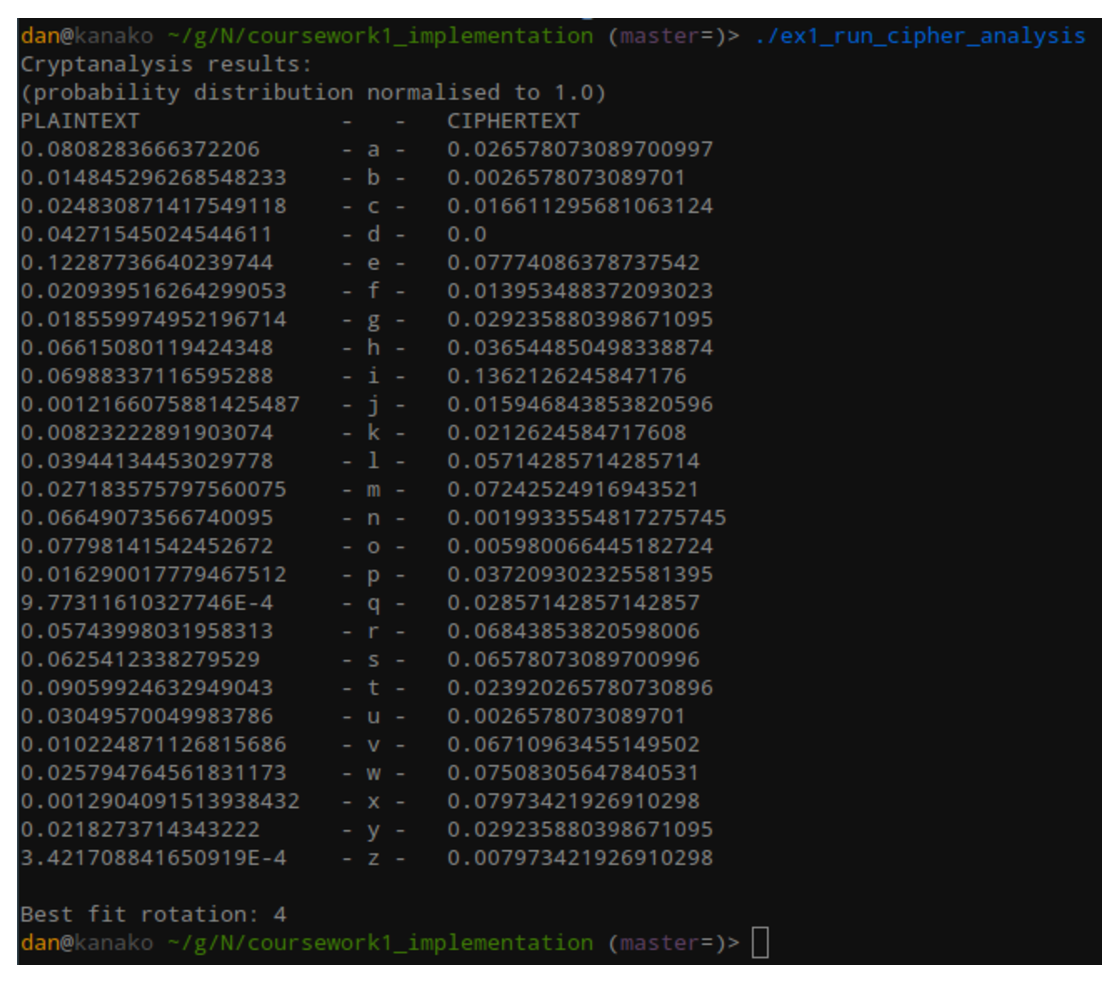
\includegraphics[width=0.65\textwidth]{graphics/ex1_cipher_analysis.eps}
  \caption{Result of automatic shift cipher detection}
  \label{fig:plaintext_output}
  \label{listing:shift_cipher_analysis_results}
\end{figure}

\section{Retrieval of the plain text}

Once the nature of the shift cipher had been discovered obtaining the original
plain text was a trivial matter of applying the inverse of the offset applied to
encrypt the text, in this case -4 (or 22).

This is implemented in the \texttt{DecipherRotation} Java class and is executed
using the \texttt{ex1\_run\_rotation\_decipher} Bash script. This provides the
output given in listing \ref{listing:plain_text}.

\begin{listing}
  \inputminted[frame=lines,fontsize=\scriptsize]{text}{../coursework1_implementation/src/test/resources/Exercise1Plaintext.txt}
  \caption{Retrieved plain text}
  \label{listing:plain_text}
\end{listing}

\printbibliography

\end{document}
